% Options for packages loaded elsewhere
\PassOptionsToPackage{unicode}{hyperref}
\PassOptionsToPackage{hyphens}{url}
%
\documentclass[
]{article}
\usepackage{amsmath,amssymb}
\usepackage{lmodern}
\usepackage{iftex}
\ifPDFTeX
  \usepackage[T1]{fontenc}
  \usepackage[utf8]{inputenc}
  \usepackage{textcomp} % provide euro and other symbols
\else % if luatex or xetex
  \usepackage{unicode-math}
  \defaultfontfeatures{Scale=MatchLowercase}
  \defaultfontfeatures[\rmfamily]{Ligatures=TeX,Scale=1}
\fi
% Use upquote if available, for straight quotes in verbatim environments
\IfFileExists{upquote.sty}{\usepackage{upquote}}{}
\IfFileExists{microtype.sty}{% use microtype if available
  \usepackage[]{microtype}
  \UseMicrotypeSet[protrusion]{basicmath} % disable protrusion for tt fonts
}{}
\makeatletter
\@ifundefined{KOMAClassName}{% if non-KOMA class
  \IfFileExists{parskip.sty}{%
    \usepackage{parskip}
  }{% else
    \setlength{\parindent}{0pt}
    \setlength{\parskip}{6pt plus 2pt minus 1pt}}
}{% if KOMA class
  \KOMAoptions{parskip=half}}
\makeatother
\usepackage{xcolor}
\IfFileExists{xurl.sty}{\usepackage{xurl}}{} % add URL line breaks if available
\IfFileExists{bookmark.sty}{\usepackage{bookmark}}{\usepackage{hyperref}}
\hypersetup{
  pdftitle={Basic Bayes},
  hidelinks,
  pdfcreator={LaTeX via pandoc}}
\urlstyle{same} % disable monospaced font for URLs
\usepackage[margin=1in]{geometry}
\usepackage{graphicx}
\makeatletter
\def\maxwidth{\ifdim\Gin@nat@width>\linewidth\linewidth\else\Gin@nat@width\fi}
\def\maxheight{\ifdim\Gin@nat@height>\textheight\textheight\else\Gin@nat@height\fi}
\makeatother
% Scale images if necessary, so that they will not overflow the page
% margins by default, and it is still possible to overwrite the defaults
% using explicit options in \includegraphics[width, height, ...]{}
\setkeys{Gin}{width=\maxwidth,height=\maxheight,keepaspectratio}
% Set default figure placement to htbp
\makeatletter
\def\fps@figure{htbp}
\makeatother
\setlength{\emergencystretch}{3em} % prevent overfull lines
\providecommand{\tightlist}{%
  \setlength{\itemsep}{0pt}\setlength{\parskip}{0pt}}
\setcounter{secnumdepth}{5}
\ifLuaTeX
  \usepackage{selnolig}  % disable illegal ligatures
\fi

\title{Basic Bayes}
\author{true}
\date{2021-09-27}

\begin{document}
\maketitle

{
\setcounter{tocdepth}{2}
\tableofcontents
}
\hypertarget{bayes-theorem}{%
\section{Bayes Theorem:}\label{bayes-theorem}}

\[P(H|D) = \frac{P(D|H) P(H)}{P(D)}\]

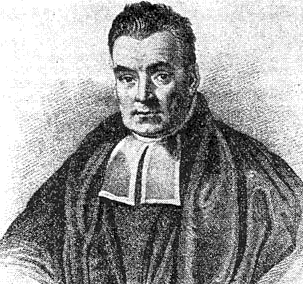
\includegraphics{../Thomas_Bayes.gif}

\hypertarget{in-words}{%
\section{In Words:}\label{in-words}}

\(\text{posterior} \propto \text{likelihood} \times \text{prior}\)

\hypertarget{benefits}{%
\section{Benefits}\label{benefits}}

\begin{enumerate}
\def\labelenumi{\arabic{enumi}.}
\item
  In Bayesian analysis, we are \emph{not} assessing the plausibility of
  the data (\(P(D|H)\)), given the assumption of a null hypothesis
  \(H_0: \text{parameter value} = 0\). This feature of Bayesian analysis
  has a few key implications:

  \begin{itemize}
  \tightlist
  \item
    We are actually estimating--\emph{the probability of a particular
    hypothesis given the data}--what we often \emph{think} we are
    estimating in Frequentist analysis. Thus, after conducting a
    Bayesian analysis, we can simply say, the probability of our
    hypothesis (\(P(H|D)\)) given the data is \emph{x} rather than
    engaging in complicated statements about ``Were the null hypothesis
    to be true, we estimate that it is \emph{p} likely that we would see
    data as extreme, or more extreme, than we actually observed.''
  \item
    Because we are directly estimating the probability of hypotheses, we
    can not only evaluate the probability of the null hypothesis
    (\(H_0\)), but also accept the null hypothesis (\(H_0\)), something
    that we are never supposed to be able to do in frequentist analysis.
    Being able to accept the null hypothesis may have implications for
    \emph{equivalency testing} and \emph{theory simplification} and may
    reduce publication bias, if we are not always looking for ways to
    reject \(H_0\).
  \end{itemize}
\item
  In Bayesian analysis, we are able to incorporate prior information
  (\(P(H)\)). Prior information may come from a number of sources:

  \begin{itemize}
  \tightlist
  \item
    Prior history of a project.
  \item
    Meta-analyses or systematic reviews of the question being
    considered.
  \item
    Expert knowledge, or community beliefs or wisdom.
  \end{itemize}
\item
  Because Bayesian estimation relies on \emph{Markov Chain Monte Carlo
  (MCMC)} simulation methods, Bayesian methods may perform better when
  there are small samples. In multilevel modeling, Bayesian methods may
  perform better
\end{enumerate}

\end{document}
